\begin{intersong}
    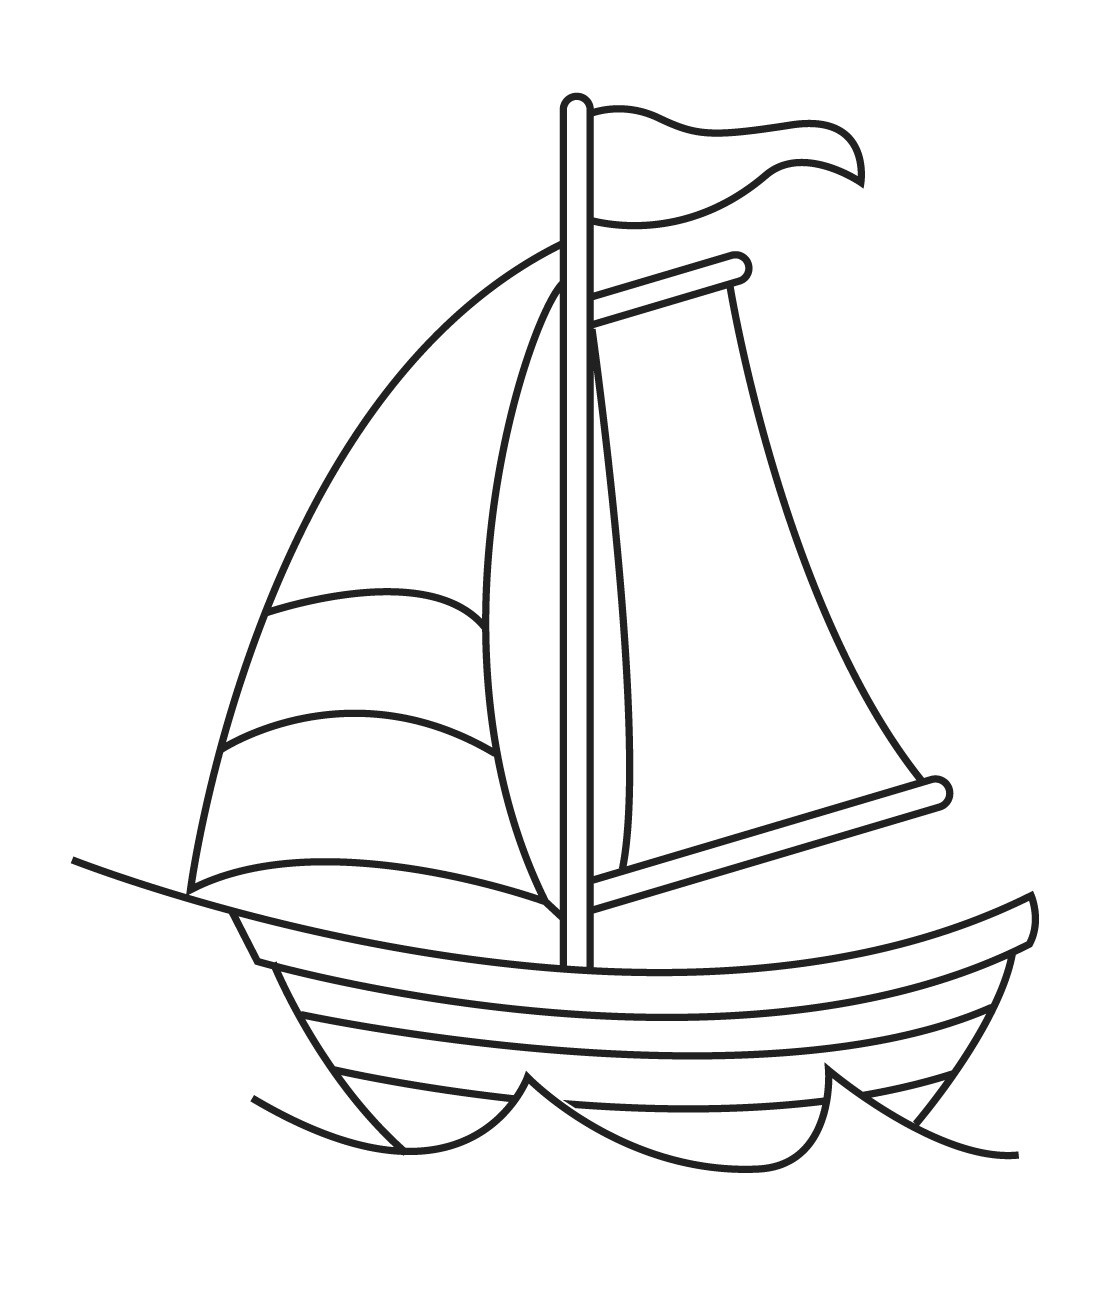
\includegraphics[width=0.4\textwidth]{vaarmaarmeekameraad}
\end{intersong}
\beginsong{Van voor naar achter}
\beginverse*
Een Nederlandse Amerikaan,
Die ziet men al van verre staan. \rep{2}
\endverse
\beginchorus
Van voor naar achter, van links naar rechts. \rep{4}
\endchorus
\beginverse*
Zijn hoofd lijkt wel op een varkenskop,
er staan maar amper drie haartjes op. \rep{2}
\endverse
\beginverse*
Zijn neus lijkt wel op een pingpongbal,
ik wou dat ik er mee spelen kan. \rep{2}
\endverse
\beginverse*
Zijn hemd lijkt wel op een prentenboek,
het hangt wel meters uit zijn broek. \rep{2}
\endverse
\beginverse*
Zijn buik lijkt wel op een luchtballon,
ik wou dat ik er in prikken kon. \rep{2}
\endverse
\endsong